\newcommand{\Ca}{\ensuremath{\mbox{Ca}^{2+}}\xspace}
\newcommand{\CaC}{\ensuremath{\left[\mbox{Ca}^{2+}\right]}\xspace}
\newcommand{\Na}{\ensuremath{\mbox{Na}^{+}}\xspace}
\newcommand{\Cl}{\ensuremath{\mbox{Cl}^{-}}\xspace}
\newcommand{\Mg}{\ensuremath{\mbox{Mg}^{2+}}\xspace}
\newcommand{\MgC}{\ensuremath{\left[\mbox{Mg}^{2+}\right]}\xspace}
\newcommand{\PEe}{\mathrm{PE}_{\mathrm{e}}}

% positional numbers
\newcommand{\kth}{\ensuremath{k^{\scriptscriptstyle\text{th}}}\xspace}
\newcommand{\nth}{\ensuremath{n^{\scriptscriptstyle\text{th}}}\xspace}

\newcommand{\Ltwo}[1]{\ensuremath{\|#1\|_{L^2}\xspace}}

\newcommand{\Dt}{\ensuremath{\Delta{}t}\xspace}
\newcommand{\Ds}{\ensuremath{\Delta{}s}\xspace}
\newcommand{\diff}[2][{}]{\dfrac{\partial #1}{\partial #2}}

\fenicschapter{A coupled stochastic and deterministic model of \Ca dynamics in the dyadic cleft}
              {A coupled stochastic and deterministic model of \Ca dynamics in the dyadic cleft}
              {A coupled stochastic and deterministic model of \Ca dynamics in the dyadic cleft}
              {Johan Hake}
              {hake}

From the time we are children we are told that we should drink milk
because it is an important source of calcium (\Ca), and that \Ca is
vital for a strong bone structure. What we do not hear as frequently
is that \Ca is one of the most important cellular messengers in the
human body \citep{AlbertsBrayLewisEtAl2002}. In particular, \Ca
controls cell death, neural signaling, secretion of different chemical
substances, the contraction of cells in the heart. The latter
is the focus of this chapter.

In this chapter, we will present a computational model that can be
used to model \Ca dynamics in a small subcellular domain called the
dyadic cleft. The model includes \Ca diffusion, which is described by
an advection-diffusion partial differential equation, and discrete
channel dynamics, which are described by stochastic Markov
models. Numerical methods implemented in DOLFIN solving the partial
differential equation will also be presented. In the last section, we
describe a time stepping scheme that is used to solve both the
stochastic and deterministic models. We will also present a solver
framework, \texttt{diffsim}, that implements this time stepping scheme
together with the numerical methods to solve the model described
above.

\section{Biological background}
\index{sarcoplasmic reticulum}
\index{ryanodine receptor}
%\index{L-type Ca channels}
\index{cell membrane} \index{excitation contraction coupling}
\index{cytosol}

In a healthy heart every heart beat originates in the sinoatrial node
where pacemaker cells trigger an electric signal. This signal is a
difference in electric potential between the interior and exterior of
the heart cells; these two domains are separated by the cell
membrane. The difference in the electric potential between these two
domains is called the membrane potential. The membrane potential
propagates through the whole heart via electrical currents which move
through the cell membrane using specific ion channels. The actively
propagating membrane potential is called an action potential. When an
action potential arrives at a specific heart cell, it triggers the
opening of L-type \Ca channels (LCCs), which bring \Ca into the
cell. Some of the \Ca diffuses over a small distance, called the
dyadic cleft, and causes further \Ca release from an intracellular \Ca
storage, the sarcoplasmic reticulum (SR), through a channel known as
the ryanodine receptor (RyR). The \Ca ions then diffuse to the main
intracellular domain of the cell, the cytosol, in which the
contractile proteins are situated. These proteins are responsible for
generating contraction in the heart cell and \Ca serves as the
trigger. The strength of the contraction is controlled by the strength
of the \Ca concentration (\CaC) in cytosol. The contraction is
succeeded by a period of relaxation caused by the extraction of \Ca
from the intracellular space by various proteins.

This chain of events is known as the Excitation Contraction (EC)
coupling \citep{Bers2001}. Several severe heart diseases can be related
to impaired EC coupling. By broadening knowledge of the EC coupling,
it may be possible to develop better treatments for such
diseases. Although grasping the big picture of EC coupling is
straightforward, it actually involves the nonlinear action of hundreds
of different protein species. Computational methods have emerged as a
natural complement to experimental studies to better understand this
process. In this chapter, we focus on the initial phase of EC
coupling wherein \Ca flows into the cell and triggers further \Ca
release.

\begin{figure}
  \centering
  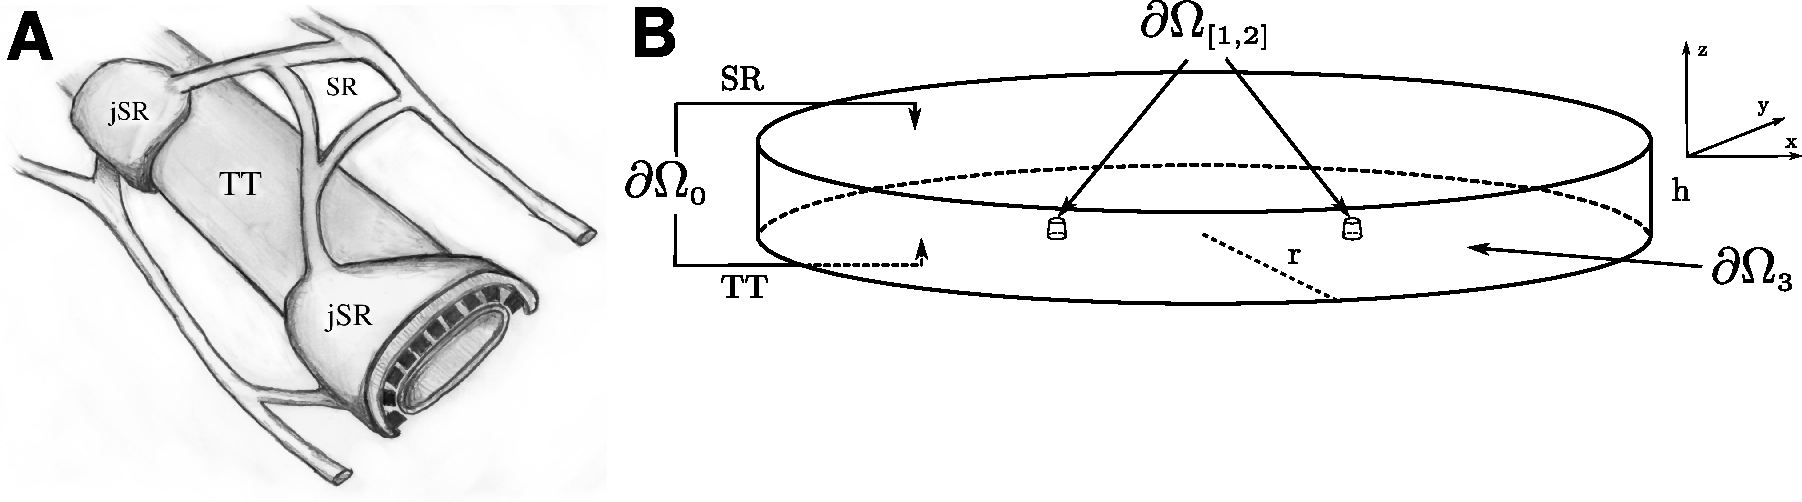
\includegraphics[width=\largefig]{chapters/hake/pdf/morphology}
  \caption[The dyadic cleft]{(A): A diagram showing the
    relationship between the TT, the SR, and the jSR in the interior
    of a heart cell. The volume between the flat jSR and the TT is the
    dyadic cleft. The black structures in the cleft are Ryanodine
    receptors, which are large channel proteins. (B): The
    geometry used for the computational model of the dyadic cleft. The
    top of the disk is the cell membrane of the SR or jSR. The bottom
    is the cell membrane of the TT, and the circumference of the disk
    is the interface to the cytosol. The elevations in the TT membrane
    model two \Ca ion channels.}
\label{fig:hake:morphology}
\end{figure}

\section{Mathematical models}
\label{sec:hake:mathematical-models}

In this section we describe the computational model for the early
phase of EC coupling. We first present the morphology of the dyadic
cleft and how we model this in our study. We then describe the
mathematical formulation for the diffusion of \Ca inside the cleft as
well for the \Ca fluxes across the boundaries. Finally, we discuss
stochastic models that govern discrete channel dynamics of the LCCs
and RyRs.

\subsection{Morphology}
\label{sec:hake:morphology}
\index{cell membrane} \index{dyadic cleft} \index{t-tubule}
\index{diffusion constant}

The dyadic cleft is the volume in the interior of the heart cell
between a structure called the t-tubule (TT) and the SR. The TT is a
network of pipe-like invaginations of the cell membrane that perforate
the heart cell \citep{SoellerCannell1999}. In
Figure~\ref{fig:hake:morphology} (A), a sketch of a small part of
a single TT together with a piece of SR is presented. Here we see that
the junctional SR (jSR) is wrapped around the TT. The small volume
between these two structures is the dyadic cleft. The space is not
well defined as it is crowded with channel proteins and varies in
size. In computational studies it is commonly approximated as a disk
or a rectangular slab
\citep{PeskoffPostLanger1992,SoellerCannell1997,KohSrinivasanChingEtAl2006,
  TanskanenGreensteinChenEtAl2007}. In this study a disk with height
$h$ = 12 nm and radius $r$ = 50 nm has been used for the domain
$\Omega$; see Figure~\ref{fig:hake:morphology} (B).

\subsection{\Ca diffusion}
\label{sec:hake:ca-diffusion}

\paragraph{Electro-diffusion.}
\index{Fick's second law} \index{screening} \index{electro-diffusion}
\index{advection-diffusion} \index{Gouy-Chapman} \index{Nernst-Planck
  equation}

We will use Fick's second law to model diffusion of \Ca in the dyadic
cleft. The diffusion constant of \Ca is set to $\sigma$ = $10^5$
nm$^2$ ms$^{-1}$ \citep{LangerPeskoff1996}. Close to the cell membrane,
ions are affected by an electric potential caused by negative charges
on the membrane
\citep{McLaughlinSzaboEisenman1971,LangnerCafisoMarceljaEtAl1990}. The
potential attenuates rapidly as it is countered by positive ions that
are attracted by the negative electrical field. This process is known
as screening. We will describe the electric potential using the
Gouy--Chapman method \citep{Grahame1947}. This theory introduces an
advection term to the standard diffusion equation, which makes the
resulting equation more difficult to solve. To simplify the
presentation, we will use a non-dimensional electric potential $\psi$,
which is the electric potential scaled by a factor of $e/kT$. Here $e$
is the electron charge, $k$ is Boltzmann's constant and $T$ is the
temperature. We will also use a non-dimensional electric field which
is given by:
\begin{equation}
  \label{eq:hake:electric_field}
  E=-\nabla\psi.
\end{equation}

The \Ca flux in a solution in the presence of an electric field is
governed by the Nernst-Planck equation,
\begin{equation}
  \label{eq:hake:nernst-planck}
  J = -\sigma\left(\nabla c-2\,cE\right),
\end{equation}
where $c = c(x,t)$ is the \CaC ($x\in\Omega$ and $t\in$[0,T]),
$\sigma$ the diffusion constant, $E = E(x)$ the non-dimensional
electric field and 2 is the valence of \Ca. Assuming conservation of
mass, we arrive at the advection-diffusion equation,
\begin{equation}
  \label{eq:hake:advection-diffusion}
  \dot{c}=\sigma\left(\Delta c + \nabla\cdot\left(2\,cE\right)\right),
\end{equation}
where $\dot{c}$ is the time derivative of $c$.

The strength of $\psi$ is defined by the amount of charge at the cell
membrane and by the combined screening effect of all the ions in the
dyadic cleft. In addition to \Ca, the intracellular solution also
contains \ensuremath{\mbox{K}^{+}}, \Na, \Cl, and \Mg. Following the
previous approach by \citet{LangnerCafisoMarceljaEtAl1990} and
\citet{SoellerCannell1997}, these other ions are treated as being in
steady state. The cell membrane is assumed to be planar and
effectively infinite. This last assumption allows us to use an
approximation of the electric potential in the solution,
\begin{equation}
  \label{eq:hake:electric_potential}
  \psi(z) = \psi_0\e^{-\kappa{}z}.
\end{equation}
Here $\psi_0$ is the non-dimensional potential at the membrane,
$\kappa$ the inverse Debye length and $z$ the distance from the cell
membrane. We will use $\psi_0=-2.2$ and $\kappa=1$ nm
\citep{SoellerCannell1997}.

\paragraph{Boundary fluxes.}
\index{stochastic channel}
\index{t-tubule}
\index{sarcoplasmic reticulum}
\index{ryanodine receptor}
%\index{L-type Ca channels}
\index{cytosol}

The boundary $\partial\Omega$ is divided into four disjoint boundaries
$\partial\Omega_k$ for $k=0,\ldots,3$; see
Figure~\ref{fig:hake:morphology} (B). To each boundary we assign
a flux, $J_{|\partial\Omega_k}=J_k$. The SR and TT membranes are
impermeable to ions, effectively making
$\partial\Omega_{\scriptscriptstyle\text{0}}$ in
Figure~\ref{fig:hake:morphology} (B) a no-flux boundary, giving us
\begin{equation}
  \label{eq:hake:no-flux}
  J_{\scriptscriptstyle 0}= 0.
\end{equation}
We include 2 LCCs in our model. The \Ca flows into the cleft at the
$\partial\Omega_{\scriptscriptstyle\text{[1,2]}}$ boundaries; see
Figure~\ref{fig:hake:morphology} (B). \Ca entering via these
channels then diffuses to the RyRs, triggering \Ca release from the
SR. This additional \Ca flux will not be included in the simulations;
however, the stochastic dynamics of the opening of the RyR channel
will be considered. The \Ca that enters the dyadic cleft diffuses into
the main compartment of cytosol, introducing a third flux. This flux
is included in the model at the
$\partial\Omega_{\scriptscriptstyle\text{3}}$ boundary.

The LCC is a stochastic channel that is either open or closed. When
the channel is open \Ca flows into the cleft. The current amplitude
of an open LCC channel is modeled to be -0.1 pA
\citep{GuiaSternLakattaEtAl2001}. The LCC flux is then,
\begin{equation}
\label{eq:hake:constant-current-flux}
J_{\scriptscriptstyle[2,3]}= \left\{
  \begin{array}{c@{\quad\quad}l}
    0,& \text{closed channel},\\
    - \frac{i}{2\,F\,A},& \text{open channel},
  \end{array}
\right.
\end{equation}
\noindent where $i$ is the amplitude, 2 the valence of \Ca, $F$
Faraday's constant and $A$ the area of the channel. Note that an
inward current is, by convention, negative.

The flux to the cytosol is modeled as a concentration-dependent flux,
\begin{equation}
  \label{eq:hake:conc-dependent-flux}
  J_{\scriptscriptstyle 3}= -\sigma\frac{c - c_0}\Ds,
\end{equation}
where $c$ is the concentration in the cleft at the boundary, $c_0$ the
concentration in the cytosol, and \Ds~is an approximation of the
distance to the center of the cytosol. In our model, we have used \Ds
= 50 nm.

\begin{figure}
  \centering
  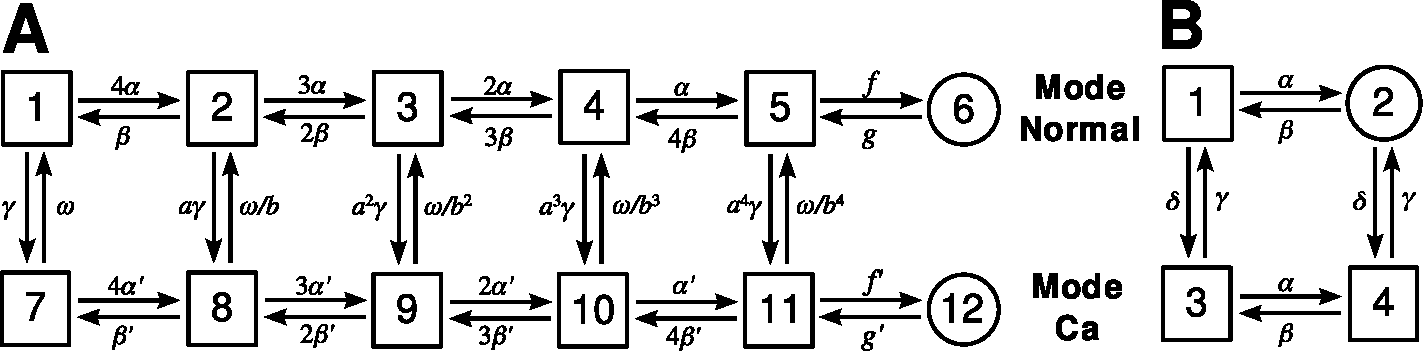
\includegraphics[height=\largefig]{chapters/hake/pdf/markov_models}
  \caption[Discrete markov models]{(A): State diagram of the
    discrete LCC Markov model from \citet{JafriRiceWinslow1998}. Each
    channel can be in one of the 12 states.  The transitions between
    the states are controlled by propensities. The $\alpha$, and
    $\beta$ are voltage-dependent, $\gamma$ is \CaC-dependent and $f$,
    $a$, $b$, and $\omega$ are constant (see
    \citet{JafriRiceWinslow1998} for further details). The channel
    operates in two modes: \textit{Mode normal}, represented by the
    states in the upper row, and \textit{Mode Ca}, represented by the
    states in the lower row. In state 6 and 12, the channel is open,
    but state 12 is rarely entered as $f'\ll{}f$, effectively making
    \textit{Mode Ca} an inactivated mode. (B): State diagram
    of an RyR from \citet{SternSongEtAl1999}. The $\alpha$ and
    $\gamma$ propensities are \Ca-dependent, representing the
    activation and inactivation dependency of the cytosolic \CaC. The
    $\beta$ and $\delta$ propensities are constant.}
  \label{fig:hake:markov-models}
\end{figure}

\subsection{Stochastic models of single channels}
\label{sec:hake:stochastic-models}
\index{stochastic channel} \index{Markov chain model} \index{Discrete
  state} \index{propensity functions}

Discrete and stochastic Markov chain models are used to describe
single channel dynamics for the LCC and RyR. Such models are described
by a certain number of discrete states. Each channel can be in any one
of these states, and a transition between two states is a stochastic
event. The frequency of these events is determined by the so called
propensity functions associated with each transition. These functions,
which may vary with time, characterize the probability per unit time
that the corresponding transition event occurs. Each Markov model
defines its own propensity functions.

\paragraph{L-type \Ca channel.}
\label{sec:hake:lcc}

%\index{L-type Ca channels}

The LCC opens when an action potential
arrives at the cell, and the channel inactivates when \Ca ions bind to
binding sites on the intracellular side of the channel. An LCC is
composed of a complex of four transmembrane subunits. Each of these
can be permissive or non-permissive. For the whole channel to be open,
all four subunits must be permissive, and the channel must then
undergo a last conformational change to the open state
\citep{Hille2001}. In this chapter, we employ a Markov model of the LCC
that incorporates voltage-dependent activation together with a
\Ca-dependent inactivation
\citep{JafriRiceWinslow1998,GreensteinWinslow2002}. The state diagram
of this model is presented in Figure~\ref{fig:hake:markov-models}
(A). It consists of 12 states, where state 6 and 12 are the
only conducting states and hence define the open states. The
transition propensities are defined by a set of functions and
constants, which are all described in \citet{GreensteinWinslow2002}.

\paragraph{Ryanodine receptors.}
\label{sec:hake:ryr}
\index{ryanodine receptor}

RyRs are \Ca specific channels that are gathered in clusters at the SR
membrane in the dyadic cleft. These clusters can consist of several
hundred RyRs
\citep{BeuckelmannWier1988,Franzini-ArmstrongProtasiRamesh1999}. They
open by single \Ca ions attaching to the receptors on the cytosolic
side. We will use a modified version of a phenomenological RyR model
that mimics the physiological functions of the channel
\citep{SternSongEtAl1999}. The model consists of four states where only
one, state 2, is conducting; see Figure~\ref{fig:hake:markov-models}
(B). The $\alpha$ and $\gamma$ propensities are \Ca-dependent,
representing the activation and inactivation dependency of cytosolic
\CaC. The $\beta$ and $\delta$ propensities are constants. For
specific values of propensities; see \citet{SternSongEtAl1999}.

\section{Numerical methods for the continuous system}

In this section we will describe the numerical methods used to solve
the continuous part of the computational model of \Ca dynamics in the
dyadic cleft. We will provide DOLFIN code for each part of the
presentation. The first part of the section describes the
discretization of the continuous problem using a finite element
method. The second part describes a method to stabilize the
discretization, and we also conduct a parameter study to find the
optimal stabilization parameters.


\subsection{Discretization}
\label{sec:hake:discretization}

The continuous problem is defined
by~(\ref{eq:hake:advection-diffusion}~-\ref{eq:hake:conc-dependent-flux})
together with an initial condition. Given a bounded domain $\Omega
\subset \Rset^3$ with the boundary $\partial\Omega$ we want to find
$c = c(x,t) \in \Rset_+$, for $x\in \Omega$ and $t \in [0,T]$, such
that:
\begin{equation}
\label{eq:hake:full_system}
\left\{
  \begin{array}{r@{\quad=\quad}ll}
    \dot{c}&\sigma\Delta c - \nabla\cdot\left(ca\right)&  \text{in } \Omega, \\
    \sigma\partial_nc-ca\cdot n&J_k& \text{on } \partial\Omega_k,\; k = 1,\ldots,4,
  \end{array}
\right.
\end{equation}
and $c(\cdot,0) = c_0(x)$. Here $a=a(x)=2\sigma E(x)$ and $J_k$ is the
\kth flux at the \kth boundary $\partial\Omega_k$, where
$\bigcup^4_{k=1}\partial\Omega_k=\partial\Omega$, $\partial_nc =
\nabla c\cdot n$, where $n$ is the outward normal on the boundary. The
$J_k$ are given by~(\ref{eq:hake:no-flux})-(\ref{eq:hake:conc-dependent-flux}).

The continuous equations are discretized using a finite element method
in space. (\ref{eq:hake:full_system}) is multiplied with a proper
test function, $v$, and integrated over the spatial domain, thus
obtaining:
\begin{equation}
  \label{eq:hake:advection-diffusion-weak-form-0}
  \int_\Omega\dot{c}v \dx = \int_\Omega \left(\sigma\Delta c-\nabla(ca)\right) v \dx.
\end{equation}
Integration by parts together with the boundary conditions
in~(\ref{eq:hake:full_system}) yields:
\begin{equation}
  \label{eq:hake:advection-diffusion-weak-form}
  \int_\Omega\dot{c}v \dx = -\int_\Omega \left(\sigma\nabla c-ca\right)\cdot\nabla v \dx + \sum_k\int_{\partial\Omega_k} J_kv \ds{}_k.
\end{equation}
Consider a mesh $\mesh = \left\{T\right\}$ of simplicial cells
$T$. Let $V_h$ denote the space of piecewise linear polynomials
defined relative to the mesh $\mesh$. Using the backward Euler methods in
time, we seek an approximation of $c$: $c_h\in V_h$ with nodal basis
$\left\{\phi_i\right\}^N_{i=1}$. (\ref{eq:hake:advection-diffusion-weak-form})
can now be discretized as follows: Consider the \nth time step, then
given $c_h^n$ find $c_h^{n+1} \in V_h$ such that
\begin{equation}
  \label{eq:hake:advection-diffusion-weak-discrete-form}
  \int_{\Omega} \frac{c_h^{n+1}-c_h^{n}}{\Dt}v \dx = -\int_{\Omega} \left(\sigma\nabla c_h^{n+1}-c_h^{n+1}a\right)\cdot\nabla v \dx + \sum_k\int_{\partial\Omega} J_kv\ds_{k},\quad\foralls v \in V_h,
\end{equation}
where \Dt is the size of the time step. The trial function $c^n_h(x)$
is expressed as a weighted sum of basis functions,
\begin{equation}
  \label{eq:hake:discrete-solution}
  c^n_h(x) = \sum^N_j C_j^n\phi_j(x).
\end{equation}
where $C_j^n$ are the coefficients. Due to the choice of $V_h$, the
number of unknowns $N$ will coincide with the number of vertices of
the mesh.

% FIXME: Rephrase 'Taking test function, v=...' below

Taking test function, $v=\phi_i$, $i\in\left\{1,\ldots,N\right\}$
gives the following algebraic system of equations in terms of the
coefficients $\left\{ c^{n+1}_i\right\}^N_{i=1}$:
\begin{equation}
  \label{eq:hake:algebraic-equation}
  \frac{1}{\Dt}\text{\bfseries\itshape M}\left(C^{n+1}-C^n\right) =  \left(-\text{\bfseries\itshape K}+\text{\bfseries\itshape E}+\sum_k\alpha^k\text{\bfseries\itshape F}^k\right)C_j^{n+1}+\sum_k c_0^k\,f^k.
\end{equation}
Here $C^n\in \Rset^N$ is the vector of coefficients from the discrete
solution, $c^n_h(x)$, $\alpha^k$ and $c_0^k$ are constant coefficients
given by (\ref{eq:hake:no-flux})--(\ref{eq:hake:conc-dependent-flux})
and\\[-1.0em]
\begin{equation}
  \renewcommand{\arraystretch}{1.7}
  \renewcommand{\baselinestretch}{1.7}
  \begin{array}{r@{\;=\;}lcr@{\;=\;}l}
    \text{\bfseries\itshape M}_{ij}&\displaystyle\int_\Omega\phi_i\phi_j \dx,& \quad\quad&\text{\bfseries\itshape K}_{ij}&\displaystyle\int_\Omega\nabla\phi_i\cdot\nabla\phi_j \dx,\\
    \text{\bfseries\itshape E}_{ij}&\displaystyle\int_\Omega a\phi_i\cdot\nabla\phi_j \dx,& \quad\quad&\text{\bfseries\itshape F}^k_{ij}&\displaystyle\int_{\partial\Omega_k}\phi_i\phi_j \ds,
  \end{array}
  \renewcommand{\arraystretch}{1}
  \renewcommand{\baselinestretch}{1}
  \label{eq:hake:matrices}
\end{equation}
are the entries in the {\bfseries\itshape M}, {\bfseries\itshape K},
{\bfseries\itshape E} and {\bfseries\itshape F}$^k$ matrices. $f^k$
are boundary source vectors corresponding to the \kth boundary, with
vector elements given by:
\begin{equation}
  \label{eq:hake:vector}
  f^k_{i}=\int_{\partial\Omega_k}\phi_i \ds.
\end{equation}

The following DOLFIN code assembles the matrices and vectors
from~(\ref{eq:hake:matrices})--(\ref{eq:hake:vector}):
\begin{python}
import numpy as np
from dolfin import *

mesh = Mesh("cleft_mesh.xml.gz")
mesh.order()

Vs = FunctionSpace(mesh, "Lagrange", 1)
Vv = VectorFunctionSpace(mesh, "Lagrange", 1)

v = TestFunction(Vs)
u = TrialFunction(Vs)

# Defining the electric field-function
a = Expression(["0.0","0.0","phi_0*valence*kappa*sigma*exp(-kappa*x[2])"],
               defaults = {"phi_0":-2.2,"valence":2,"kappa":1,"sigma":1.e5},
               element=Vv.ufl_element())

# Assembly of the K, M and A matrices
K = assemble(inner(grad(u), grad(v))*dx)
M = assemble(u*v*dx)
E = assemble(-u*inner(a, grad(v))*dx)

# Collecting face markers from a file, and skip the 0 one
sub_domains = MeshFunction("uint", mesh, "cleft_mesh_face_markers.xml.gz")
unique_sub_domains = list(set(sub_domains.values()))
unique_sub_domains.remove(0)

# Assemble matrices and source vectors from exterior facets domains
domain = MeshFunction("uint", mesh, 2)
F = {}; f = {}; tmp = K.copy(); tmp.zero()
for k in unique_sub_domains:
    domain.values()[:] = (sub_domains.values() != k)
    F[k] = assemble(u*v*ds, exterior_facet_domains = domain,
                    tensor = tmp.copy(), reset_sparsity = False)
    f[k] = assemble(v*ds, exterior_facet_domains = domain)
\end{python}
In the above code we define only one form for the different boundary
mass matrices and boundary source vectors, \texttt{u*v*ds} and
\texttt{v*ds}, respectively. The \texttt{assemble} routine will
assemble these forms over the $0^{\scriptscriptstyle\text{th}}$
subdomain. By passing subdomain specific \texttt{MeshFunction}s to
the assemble routine, we can assemble the correct boundary mass
matrices and boundary source vectors. We collect the matrices and
boundary source vectors; these are then added to form the linear
system to be solved at each time step. If an LCC opens, the collected
source vector from that boundary will contribute to the right-hand
side. If an LCC closes the same source vector are removed from the
right-hand side. When an LCC either opens or closes, a large flux is
either added to or removed from the system. To be able to resolve
sharp time gradients correctly we need to take smaller time steps
following such an event. After the time step has been reset to a small
number we can start expanding it by multiplying the time step with a
constant $>$ 1.

The sparse linear system is solved using the \petsc linear algebra
backend \citep{BalayBuschelmanGroppEtAl2001} in DOLFIN together with
the Bi-CGSTAB iterative solver \citep{Vorst1992}, and the BoomerAMG
preconditioners from hypre \citep{FalgoutYang2002}. A script that
solves the algebraic system from~(\ref{eq:hake:algebraic-equation})
together with a crude time stepping scheme for the opening and closing
of the included LCC channel is presented below.

\subsection{Stabilization}
\label{sec:hake:stabilization}
\index{stabilization}
\index{stabilization!Streamline upwind Petrov-Galerkin}
\index{stabilization!parameter}
\index{stabilization!element P\'eclet number}
\index{tetgen}

It turns out that the algebraic system
in~(\ref{eq:hake:algebraic-equation}) can be numerically unstable for
physiological relevant values of $a$. This is due to the transport
term introduced by {\bfseries\itshape E}$_{ij}$
from~(\ref{eq:hake:matrices}). We have chosen to stabilize the system
using the Streamline upwind Petrov-Galerkin (SUPG) method
\citep{BrooksHughes1982}. This method adds an upwind discontinuous
contribution to the test function in the streamline
direction~(\ref{eq:hake:advection-diffusion-weak-form-0}):
\begin{equation}
  \label{eq:hake:stabilizing-term}
  v' = v+s, \text{ where } s = \tau\frac{h\tau_e}{2\|a\|}a\cdot\nabla v.
\end{equation}
Here $\tau$ is a parameter we want to optimize (see later in this
Section), $\|\cdot\|$ is the Euclidean norm in $\Rset^3$, $h=h(x)$ is
the element size, and $\tau_e=\tau_e(x)$, is given by,
\begin{equation}
  \label{eq:hake:element-tau}
  \tau_e=\coth(\PEe)-\frac{1}{\PEe},
\end{equation}
where $\PEe$ is the element P\'eclet number:
\begin{equation}
  \label{eq:hake:peclet}
  \PEe = \frac{\|a\|h}{2\sigma}.
\end{equation}
When $\PEe$ is larger than 1 the system becomes unstable, and
oscillations are introduced.

In the 1D case with a uniform mesh, the stabilization term defined
by~(\ref{eq:hake:element-tau})--(\ref{eq:hake:peclet}) can give exact
nodal solutions
\citep{ChristieGriffithsMitchellEtAl1976,BrooksHughes1982}. Our choice
of stabilization parameter is inspired by this.  We have used $h$ to
denote the diameter of the sphere that circumscribes the local
tetrahedron.  This is what \dolfin implements in the function
\texttt{Cell.diameter()}. We recognize that other choices exist, which
might give improved stabilization \citep{JohnKnobloch2007}; for
example \citet{TezduyarPark1986} use a length based on the size of the
element in the direction of $a$.

The DOLFIN code that assembles the SUPG part of the problem is
presented in the following script:
\begin{python}
# Python code for the assembly of the SUPG term for the mass and advection matrices
# Defining the stabilization using local Peclet number
cppcode = """class Stab : public Expression {
public:
  GenericFunction* field; double sigma;
  Stab(): Expression(3), field(0), sigma(1.0e5){}
  void eval(Array<double>& v, const Data& data) const {
    if (!field)
      error("Attach a field function.");
    double field_norm = 0.0; double tau = 0.0;
    double h = data.cell().diameter();
    field->eval(v, data);
    for (uint i = 0;i < data.x.size(); ++i)
      field_norm += v[i]*v[i];
    field_norm = sqrt(field_norm);
    double PE = 0.5*field_norm * h/sigma;
    if (PE > DOLFIN_EPS)
      tau = 1/tanh(PE)-1/PE;
    for (uint i = 0;i < data.x.size(); ++i)
      v[i] *= 0.5*h*tau/field_norm;
}};
"""
stab = Expression(cppcode); stab.field = a

# Assemble the stabilization matrices
E_stab = assemble(div(a*u)*inner(stab, grad(v))*dx)
M_stab = assemble(u*inner(stab, grad(v))*dx)

# Adding them to the A and M matrices, weighted by the global tau
tau = 0.28; E.axpy(tau, E_stab, True); M.axpy(tau, M_stab,True)
\end{python}
In the above script, two matrices \texttt{E\_stab} and
\texttt{M\_stab} are assembled. Both matrices are added to the
corresponding advection and mass matrices \texttt{E} and \texttt{M},
weighted by the global parameter \texttt{tau}.

A mesh with finer resolution close to the TT surface, at $z=0$ nm, is
used to resolve the steep gradient of the solution in this area. It is
here the electric field is at its strongest yielding an element
P\'eclet number larger than 1. However the field attenuates quickly: at
$z=3$ nm the field is down to 5\% of the maximum amplitude, and at
$z=5$ nm it is down to 0.7\%. The mesh can thus be fairly coarse in
the interior of the domain. The mesh generator \texttt{tetgen} is used
to to produce meshes with the required resolution \citep{Si2007}.

\begin{figure}
  \centering
  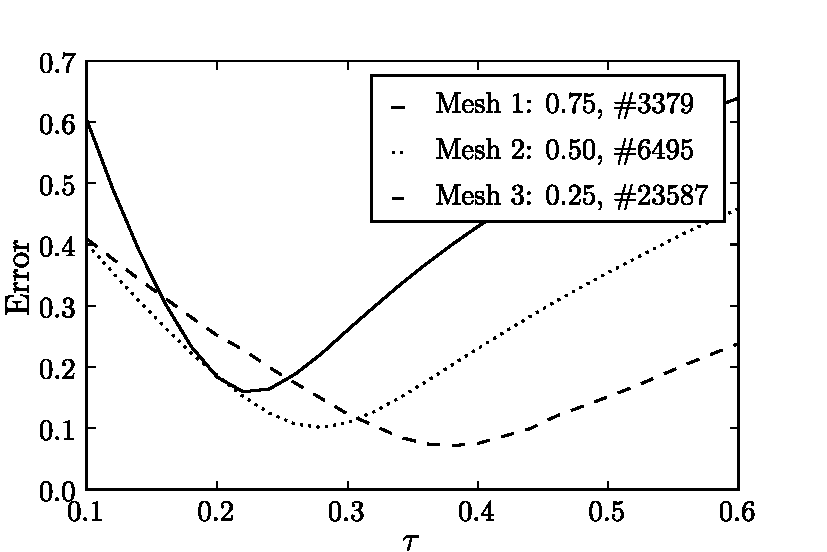
\includegraphics[width=\largefig]{chapters/hake/pdf/error_plot}
  \caption[Error plot]{The figure shows a plot of the error versus the
    stabilization parameter $\tau$ for 3 different mesh
    resolutions. The mesh resolutions are given by the median of the
    $z$ distance of all vertices and the total number of vertices in
    the mesh; see legend. We see that the minimal values of the error
    for the three meshes occur at three different $\tau$: $0.22$, $0.28$,
    and~$0.38$.}
  \label{fig:hake:error_plot}
\end{figure}

\subsection{Solving the discretized system}

The DOLFIN code that solves the discretized and stabilized system
from~(\ref{eq:hake:algebraic-equation}) is given by:
\begin{python}
# Model parameters
dt_min = 1.0e-10; dt = dt_min; t = 0; c0 = 0.1; tstop = 1.0
events = [0.2,tstop/2,tstop,tstop]; dt_expand = 2.0;
sigma = 1e5; ds = 50; area = pi; Faraday = 0.0965; amp = -0.1
t_channels = {1:[0.2,tstop/2], 2:[tstop/2,tstop]}

# Initialize the solution Function and the left and right-hand side
u = Function(Vs); x = u.vector()
x[:] = c0*exp(-a.valence*a.phi_0*exp(-a.kappa*mesh.coordinates()[:,-1]))
b = Vector(len(x)); A = K.copy();

solver = KrylovSolver("bicgstab","amg_hypre")
solver.parameters["relative_tolerance"] = 1e-10
solver.parameters["absolute_tolerance"] = 1e-7

plot(u, vmin=0, vmax=4000, interactive=True)
while t < tstop:
    # Initalize the left and right-hand side
    A.assign(K); A *= sigma; A += E; b[:] = 0

    # Adding channel fluxes
    for c in [1,2]:
        if t >= t_channels[c][0] and t < t_channels[c][1]:
            b.axpy(-amp*1e9/(2*Faraday*area),f[c])

    # Adding cytosole flux at Omega 3
    A.axpy(sigma/ds,F[3],True); b.axpy(c0*sigma/ds,f[3])

    # Applying the Backward Euler time discretization
    A *= dt; b *= dt; b += M*x; A += M

    solver.solve(A,x,b)
    t += dt; print "Ca Concentration solved for t:",t

    # Handle the next time step
    if t == events[0]:
        dt = dt_min; events.pop(0)
    elif t + dt*dt_expand > events[0]:
        dt = events[0] - t
    else:
        dt *= dt_expand

    plot(u, vmin=0, vmax=4000)

plot(u, vmin=0, vmax=4000, interactive=True)
\end{python}
The time stepping scheme presented in the above code is crude, but
simple and explicit. The solution algorithm is based on pre-assembled
matrices. Adding matrices and vectors together makes the construction
of the linear system more complicated compared to including the time
discretization directly into a variational form. However, by
pre-assemble the matrices and source vectors we do not have to
reassemble the linear system during the time stepping, and time is
saved during execution. This becomes important when larger meshes and
hundred of channels are included.
\begin{figure}
  \centering
  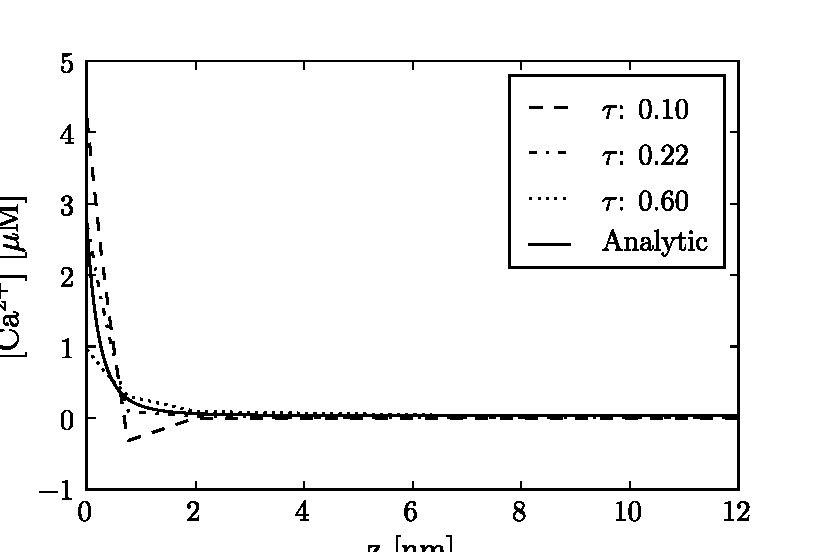
\includegraphics[width=\largefig]{chapters/hake/pdf/traces_mesh_1}
  \caption[Concentration traces 1]{The figure shows concentration
    results from numerical solutions from Mesh 1 (see legend of
    Figure~\ref{fig:hake:error_plot}), for three different $\tau$,
    together with the analytical solution. The solutions were picked
    from a line between the points (0,0,0) and (0,0,12). We see that
    the solution with $\tau=0.10$ oscillates. The solution with
    $\tau=0.22$ was the solution with smallest global error for this
    mesh (see Fig~\ref{fig:hake:error_plot}), and the solution with
    $\tau=0.60$ undershoots the analytical solution at $z=0$ nm with
    $\simeq$1.7 $\mu$M.}
  \label{fig:hake:traces_mesh_1}
\end{figure}

\begin{figure}
  \centering
  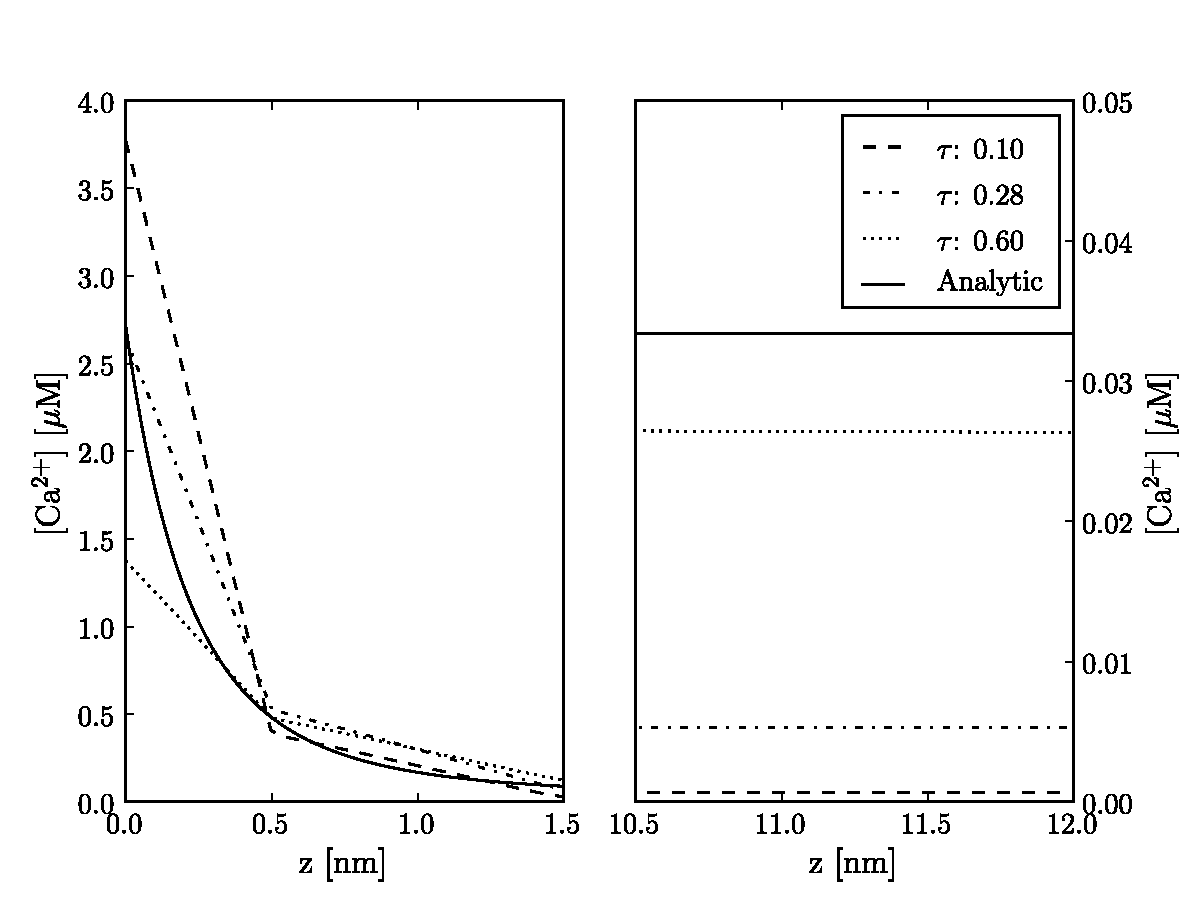
\includegraphics[width=\largefig]{chapters/hake/pdf/traces_mesh_2}
  \caption[Concentration traces 2]{The figures show the
    concentration traces of the numerical solutions from Mesh 2 (see
    legend of Figure~\ref{fig:hake:error_plot}), for three different
    $\tau$, together with the analytical solution. The solution traces
    in the two panels are picked from a line between the points
    (0,0,0) and (0,0,1.5), for the left panel, and between spatial
    points (0,0,10.5) and (0,0,12) for the right panel. We see from
    both panels that the solution for $\tau=0.10$ gives the poorest
    approximation. The solution with $\tau=0.28$ was the solution
    with smallest global error for this mesh (see
    Fig~\ref{fig:hake:error_plot}), and this is reflected in the
    reasonable good fit seen in the left panel, especially at $z=0$
    nm. The solution with $\tau=0.60$ undershoots the analytical
    solution at $z=0$ with $\simeq$1.2 $\mu$M. From the right panel
    we see that all numerical solutions undershoot at $z=12$ nm. We
    also see that the trace for $\tau=0.60$ comes the closest to the
    analytical solution.}
  \label{fig:hake:traces_mesh_2}
\end{figure}

\subsection{Finding an optimal stabilization parameter}
The global stabilization parameter, $\tau$, is problem-dependent. To
find an optimal $\tau$ for a certain electric field and mesh, the
system in~(\ref{eq:hake:algebraic-equation}) is solved to steady
state, defined as $T = 1.0\,\mathrm{ms}$, using only homogeneous
Neumann boundary conditions. A homogeneous concentration of $c_0=0.1$
$\mu$M is used as the initial condition. The numerical solution is
then compared with the analytical solution of the problem. This solution
is acquired by setting $J=0$ in~(\ref{eq:hake:nernst-planck}) and
solving for the $c$, with the following result:
\begin{equation}
  \label{eq:hake:analytic-solution}
  c(z) = c_b\e^{-2\psi(z)}.
\end{equation}
Here $\psi$ is given by~(\ref{eq:hake:electric_potential}), and
$c_b$ is the bulk concentration; that is, where $z$ is large. $c_b$ was
chosen such that the integral of the analytical solution was equal to
$c_0\times V$, where $V$ is the volume of the domain.

The error of the numerical solution for different values of $\tau$ and
for three different mesh resolutions is plotted in
Figure~\ref{fig:hake:error_plot}. The meshes are enumerated from 1-3,
and a higher number corresponds to a better resolved boundary layer at
z=0 nm. As expected, we see that the mesh that resolves the boundary
layer best produces the smallest error. The error is computed using
the $L^2(\Omega)$ norm and is normalized by the $L^2(\Omega)$ norm of
the analytical solution,
\begin{equation}
  \label{eq:hake:error_norm}
  \frac{\Ltwo{c(T)-c_h^{n_T}}}{\Ltwo{c(T)}},
\end{equation}
where $n_T$ is the time step at $t=T$. The mesh resolutions are
quantified by the number of vertices close to $z=0$. In the legend of
Figure~\ref{fig:hake:error_plot}, the median of the $z$ distance of all
vertices and the total number of vertices in each mesh is presented.

Traces from the actual simulations are plotted in
Figure~\ref{fig:hake:traces_mesh_1}-\ref{fig:hake:traces_mesh_3}. In
each figure are three numerical and one analytical solution plotted
for each mesh. The numerical solutions are from simulations using
three different $\tau$: 0.1, 0.6 and the $L^2$-optimal $\tau$ (see
Figure~\ref{fig:hake:error_plot}). The traces in the figures are from
the discrete solution $c_h^{n_T}$, interpolated onto the straight line
between the spatial points $p_0$=(0,0,0) and $p_1$=(0,0,12).

\begin{figure}
  \centering
  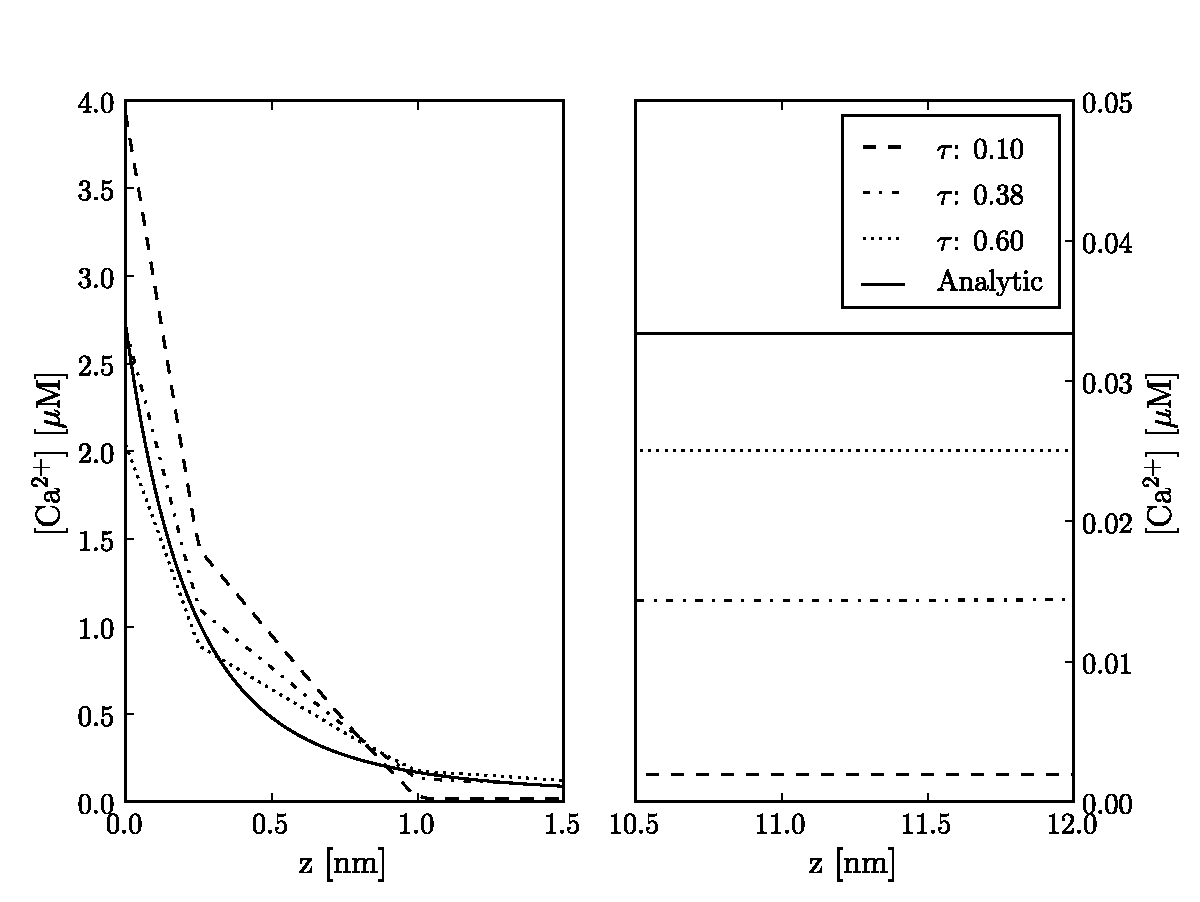
\includegraphics[width=\largefig]{chapters/hake/pdf/traces_mesh_3}
  \caption[Concentration traces 3]{The figure shows the
    concentration traces of the numerical solutions from Mesh 3 (see
    legend of Figure~\ref{fig:hake:error_plot}), for three different
    $\tau$, together with the analytical solution. The traces in the
    two panels were picked from the same lines for
    Figure~\ref{fig:hake:traces_mesh_2}. Again, we see from both
    panels that the solution with $\tau=0.10$ give the poorest
    solution. The solution with $\tau=0.38$ was the solution with
    smallest global error for this mesh (see
    Fig~\ref{fig:hake:error_plot}), and this is reflected in the
    good fit seen in the left panel, especially at $z=0$nm. The
    solution with $\tau=0.60$ undershoots the analytical solution at
    $z=0$ with $\simeq$0.7 $\mu$M. From the right panel, we see that
    all numerical solutions undershoot at $z=15$ nm, and the trace
    with $\tau=0.60$ here also comes closest to the analytical
    solution.}
  \label{fig:hake:traces_mesh_3}
\end{figure}

In Figure~\ref{fig:hake:traces_mesh_1} the traces from Mesh 1 are
plotted. Here we see that the numerical solutions are quite poor for
some $\tau$. The solution with $\tau=0.10$ is not correct as it
produces negative concentrations; a physiological impossibility. The
solution with $\tau=0.60$ seems more correct, but it undershoots the
analytical solution at $z=0$ with $\simeq$1.7 $\mu$M. The solution with
$\tau=0.22$ is the $L^2$-optimal solution for Mesh 1, and approximates
the analytical solution at $z=0$ well.

In Figure~\ref{fig:hake:traces_mesh_2}, the traces from Mesh 2 are
presented in two plots. The left plot shows the traces for $z<1.5$ nm,
and the right shows traces for $z>10.5$ nm. In the left plot, we see
the same tendency as in Figure~\ref{fig:hake:traces_mesh_1}: an
overshoot of the solution with $\tau=0.10$ and an undershoot of the
solution with $\tau=0.60$. The $L^2$-optimal solution for $\tau=0.28$,
overshoots the analytical solution for the shown interval in the left
plot, but undershoots for the rest of the trace.

In the last figure, Figure~\ref{fig:hake:traces_mesh_3}, traces from
mesh 3 are presented. The results are also presented in two plots
here, corresponding to the same $z$ interval as in
Figure~\ref{fig:hake:traces_mesh_2}. We see that the solution with
$\tau=0.10$ is again not acceptable in either interval. In the left
plot, it clearly overshoots the analytical solution for most of the
interval, and then undershoot the analytical solution for the rest of
the interval. The solution with $\tau=0.60$ is improved here compared
to the two previous plots. It undershoots the analytical solution at
$z=0$; but stays closer for the rest of the interval as compared to
the $L^2$-optimal solution. The $L^2$ norm penalizes larger distances
between two traces; that is, weighting the error close to $z=0$ more
than the rest. The optimal solution measured in the Max norm is given
when $\tau=50$ (result not shown).

The numerical results tell us that the Streamline upwind
Petrov-Galerkin method can be used to stabilize the Finite element
solution of the advection-diffusion problem presented
in~(\ref{eq:hake:full_system}). Three different meshes that resolve
the boundary layer at $z=0\,\mathrm{nm}$ differently were used. For
each mesh a global $\tau$, which produce an $L^2$ optimal solution,
were obtained. To test convergence rate we also did simulations with
homogeneously refined meshes. The largest mesh had $\simeq$180 000
number of vertices. The errors for the optimal $\tau$ for each mesh
resolution were compared and linear convergence rate was obtained
(result not shown).

The largest mesh in our test problems, the one that resolves the
boundary layer best, is not large: $\simeq$ 24 000 vertices. The
convergence study we performed showed that we could decrease the
reported error more by using meshes with better resolution. However,
the meshes we ran our simulations on, where physiological small
meshes; radius=20nm. A relevant size would need a radius of
$\simeq$200 nm. This would create a mesh with $\simeq$2.5 million
vertices for the highest resolution we use in this chapter. A mesh
with such a size would be a challenge for a serial solver, and
parallel solvers need to be employed. The software that will be
presented next, \texttt{diffsim}, does unfortunately not support
parallel solvers.

\begin{figure}
  \centering
  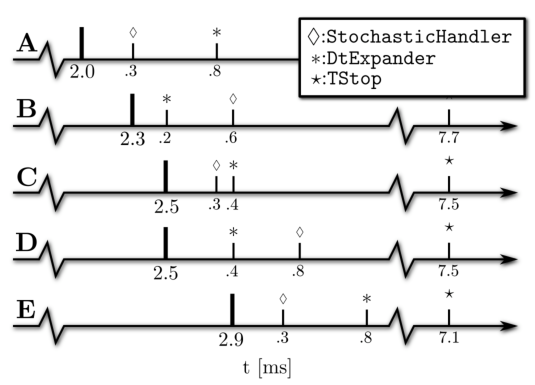
\includegraphics[width=\smallfig]{chapters/hake/pdf/timeline}
  \caption[Time stepping algorithm]{Diagram for the time stepping
    algorithm using 3 discrete objects: \texttt{DtExpander},
    \texttt{StochasticHandler}, \texttt{TStop}. The values below the
    small ticks corresponds to the time to the next event for each of
    the discrete objects. This time is measured from the last realized
    event, which is denoted by the thicker tick. See text for details.}
  \label{fig:hake:time-line}
\end{figure}

\section{\texttt{diffsim} an event-driven simulator}
\label{sec:hake:diffsim}
\index{time stepping} \index{\texttt{diffsim}} \index{FEniCS Apps} In
the DOLFIN scripts above, we show how a simple continuous solver can
be built with DOLFIN. By pre-assembling the matrices
from~(\ref{eq:hake:matrices}), a flexible system for adding and
removing boundary fluxes corresponding to the state of the channels
can be constructed. The solving script uses fixed time points for the
channel state transitions. At these time points, we minimize \Dt so we
can resolve the sharp time gradient. In between the channel
transitions we expand \Dt. This simplistic time stepping scheme has
been sufficient to solve the presented example. However, it would be
difficult to extend this to incorporate the time stepping involved
with the solution of stochastic Markov models and other discrete
variables. For such scenarios, an event-driven simulator called
\texttt{diffsim} has been developed. In the final subsections in this
chapter the algorithm underlying the time stepping scheme in
\texttt{diffsim} will be presented. An example of how one can use
\texttt{diffsim} to describe and solve a model of \Ca dynamics in the
dyadic cleft is also demonstrated.

\subsection{Stochastic system}

\label{sec:hake:stochastic-system}
\index{Gillespie method} \index{Markov chain model} \index{propensity
  function} \index{channel transition} The stochastic evolution of the
Markov chain models presented in Section
\ref{sec:hake:stochastic-models} is determined by a modified Gillespie
method \citep{Gillespie1977}, which resembles one presented in
\citet{RudigerShuaiHuisingaEtAl2007}. Here we will not go into detail,
but rather focus on the part of the method that has importance for the
overall time stepping algorithm.

The solution of the included stochastic Markov chain models is stored
in a state vector \texttt{S}. Each element in \texttt{S} corresponds
to one Markov model, and the value reflects which state each model is
in. The transitions between these states are modeled stochastically
and are computed using a modified Gillespie method. Basically this
method gives us which of the states in \texttt{S} changes to what
state and when. Not all such state transitions are relevant for the
continuous system. A transition between two closed states in the LCC
model, for instance, will not have any impact on the boundary fluxes,
and can be ignored. Only transitions that either open or close a
channel (channel transitions), will be recognized. The modified
Gillespie method assumes that any continuous variables on which a
certain propensity function depends are constant during a time
step. The error incurred by this assumption is reduced by taking
smaller time steps right after a channel transition as the continuous
field is indeed changing dramatically during this time period.

\subsection{Time stepping algorithm}
\label{sec:hake:event-driven-simulator}

To simplify the presentation of the time stepping algorithm, we only
consider one continuous variable, the \Ca field. A
\packagefont{Python}-like pseudo code for the time stepping algorithm
is shown in the following script:
\begin{python}
# Python-like pseudo code for the time stepping algorithm used in diffsim
while not stop_sim:
    # The next event
    event = min(discrete_objects)
    dt = event.next_time()

    # Step the event and check result
    while not event.step():
        event = min(discrete_objects)
        dt = event.next_time()

    # Update the other discrete objects with dt
    for obj in discrete_objects:
        obj.update_time(dt)

    # Solve the continuous equation
    ca_field.solve(dt)
    ca_field.send()

    # Distribute the event
    event.send()
\end{python}
The framework presented with this pseudo code can be expanded to
handle several continuous variables. We define a base class called
\texttt{DiscreteObject}, which defines the interface for all discrete
objects. A key function of a discrete object is to know when its
\textit{next event} is due. The \texttt{DiscreteObject} that has the
smallest next event time gets to define the size of the next \Dt. In
\packagefont{Python}, this is easily achieved by making the
\texttt{DiscreteObject}s sortable with respect to their next event
time. All \texttt{DiscreteObject}s are then collected in a list
\texttt{discrete\_objects} (see script below). The
\texttt{DiscreteObject} with the smallest next event time is then
simply \texttt{min(discrete\_objects)}. An event from a
\texttt{DiscreteObject} that does not have an impact on the continuous
solution will be ignored; for example, a Markov chain model transition
that is not a channel transition as noted above. A transition needs to
be realized before we can tell if it is a channel transition or
not. This is done by \textit{stepping} the \texttt{DiscreteObject};
that is, calling the object's \texttt{step()} method. If the method
returns \texttt{False} it will not affect the \Ca field. We then enter
a while loop and a new \texttt{DiscreteObject} is picked. If the
object returns \texttt{True} when stepped we exit the loop and
continue. Next, we have to update the other discrete objects with the
chosen \Dt, solve for the \Ca field, broadcast the solution, and last
but not least, execute the discrete event that is scheduled to happen
at \Dt.

In Figure~\ref{fig:hake:time-line}, we show an example of a possible
realization of this algorithm. In (A) we have realized a
time event at $t=2.0\,\mathrm{ms}$. The next event to be realized is a
stochastic transition, the one with smallest value below the ticks. In
(B) this event is realized, and the \texttt{StochasticHandler}
now shows a new next event time. The event is a channel transition
forcing the dt, controlled by the \texttt{DtExpander}, to be
minimized. \texttt{DtExpander} now has the smallest next event time,
and is realized in (C). The channel transition that was
realized in (B) raised the \CaC in the cleft, which in turn
increased the \Ca-dependent propensity functions in the included
Markov models. The time to next event time of the
\texttt{StochasticHandler} has therefore been updated, and moved
forward in (C). Also note that the \texttt{DtExpander} has
expanded its next event time. In (D), the stochastic transition
is realized and updated with a new next event time, but it is ignored
as it is not a channel transition. The smallest time step is now the
\texttt{DtExpander}, and this is realized in (E). In this
example, we do not realize the \texttt{TStop} event, as it is too far
away.

\subsection{\texttt{diffsim}: an example}
\index{\texttt{diffsim}} \index{event-driven simulator}

\texttt{diffsim} is a versatile, event-driven simulator that
incorporates the time stepping algorithm presented in the previous
section together with the infrastructure to solve models with one or
more diffusional domains defined by a computational mesh. Each such
domain can have several diffusive ligands. Custom fluxes can easily be
included through the framework. The submodule \texttt{dyadiccleft}
implements some published Markov models that can be used to simulate
the stochastic behavior of a dyad and some convenient boundary
fluxes. It also implements the field flux from the lipid bi-layer
discussed in Section~\ref{sec:hake:ca-diffusion}. The following script
runs 10 simulations to collect the time to release, also called the
latency, for a dyad:
\begin{python}
# An example of how diffsim can be used to simulate the time to RyR release latency, from
# a small dyad who's domain is defined by the mesh in the file cleft_mesh_with_RyR.xml.gz
from diffsim import *
from diffsim.dyadiccleft import *
from numpy import exp, from file

# Model parameters
c0_bulk = 0.1; D_Ca = 1.e5; Ds_cyt = 50; phi0 = -2.2; tau = 0.28
AP_offset = 0.1; dV = 0.5, ryr_scale = 100; end_sim_when_opend = True

# Setting boundary markers
LCC_markers = range(10,14); RyR_markers = range(100,104); Cyt_marker = 3

# Add a diffusion domain
domain = DiffusionDomain("Dyadic_cleft","cleft_mesh_with_RyR.xml.gz")
c0_vec = c0_bulk*exp(-VALENCE[Ca]*phi0*exp(-domain.mesh().coordinates()[:,-1]))

# Add the ligand with fluxes
ligand = DiffusiveLigand(domain.name(),Ca,c0_vec,D_Ca)
field  = StaticField("Bi_lipid_field",domain.name())
Ca_cyt = CytosolicStaticFieldFlux(field,Ca,Cyt_marker,c0_bulk,Ds_cyt)

# Adding channels with Markov models
for m in LCC_markers:
    LCCVoltageDepFlux(domain.name(), m, activator=LCCMarkovModel_Greenstein)
for m in RyR_markers:
    RyRMarkovModel_Stern("RyR_%d"%m, m, end_sim_when_opend)

# Adding a dynamic voltage clamp that drives the LCC Markov model
AP_time = fromfile("AP_time_steps.txt",sep="\n")
dvc = DynamicVoltageClamp(AP_time,fromfile("AP.txt",sep="\n"),AP_offset,dV)

# Get and set parameters
params = get_params()

params.io.save_data = True
params.Bi_lipid_field.tau = tau
params.time.tstop = AP_time[-1] + AP_offset
params.RyRMarkovChain_Stern.scale = ryr_scale

info(str(params))

# Run 10  simulations
data = run_sim(10,"Dyadic_cleft_with_4_RyR_scale")
mean_release_latency = mean([ run["tstop"] for run in data["time"]])
\end{python}
The two Markov models presented in Section
\ref{sec:hake:stochastic-models} are here used to model the stochastic
dynamics of the RyRs and the LCCs. The simulation is driven by a
so-called dynamic voltage clamp. With a voltage clamp we can
dynamically clamp the voltage to a certain wave form. The wave form
can be acquired from experiments. The data that define the voltage
clamp are read from a file using utilities from NumPy Python packages.

\section{Discussion}

We have presented a computational model of \Ca dynamics of the dyadic
cleft in heart cells. It consists of a coupled stochastic and
continuous system. We have showed how one can use DOLFIN to discretise
and solve the continuous system using a finite element method. Because
the continuous system is an advection-diffusion equation that produces
unstable discretizations, we investigate how one can use the SUPG
method for stability. We employ three different meshes each with
different resolutions at the boundary layer of the electrical
potential, and find an $L^2$-optimal global stabilization parameter
$\tau$ for each mesh.

We do not present a solver for the stochastic system. However, we
outline a time stepping scheme that can be used to couple the
stochastic solver with solver presented for the continuous system. A
simulator \texttt{diffsim} is briefly introduced, which implements the
presented time stepping scheme together with the presented solver for
the continuous system.
